% **************************************************************************************************************
\RequirePackage{silence} % :-\
    \WarningFilter{scrreprt}{Usage of package `titlesec'}
    \WarningFilter{scrreprt}{Activating an ugly workaround}
    \WarningFilter{titlesec}{Non standard sectioning command detected}
\documentclass[ twoside,openright,titlepage,numbers=noenddot,%1headlines,
                headinclude,footinclude,cleardoublepage=empty,abstract=on,
                BCOR=5mm,paper=a5,fontsize=11pt
                ]{scrreprt}
% \documentclass[11pt,paper=a5,footinclude,headinclude]{scrbook} % KOMA-Script book

%********************************************************************
% Note: Make all your adjustments in here
%*******************************************************
% \input{classicthesis-config}
% File encoding
\usepackage[utf8]{inputenc}

% Languages
\usepackage[main=english,ngerman]{babel}

% classicthesis setup
\PassOptionsToPackage{%
  %drafting,%
  %dottedtoc,%
  eulerchapternumbers,
  %listings,%
  %parts,%
  floatperchapter, pdfspacing,%
  beramono,%
  %minionprospacing,
  %subfig,%
  %eulermath,%
  a5paper,%
}{classicthesis}

% Meta
%
% Document information
%
\newcommand{\myTitle}{%
  Eine neue Bestimmung der Moleküldimensionen\xspace%
}
\newcommand{\mySubtitle}{
   \xspace
  }
\newcommand{\myPlainTitle}{%
  Eine neue Bestimmung der Moleküldimensionen\xspace%
}

\newcommand{\myDissNumber}{?}
\newcommand{\myName}{Albert Einstein\xspace}
\newcommand{\myUni}{\protect{ETH Z\"urich}\xspace}
\newcommand{\myLocation}{Z\"urich\xspace}
\newcommand{\myTime}{1905\xspace}

% DOI
\newcommand{\myDOI}{10.3929/ethz-a-}

% Work version info
\newcommand{\worktodo}[1]{\textcolor{red}{\textbf{TODO}: #1}}
\usepackage{scrtime}
\newcommand{\workdraft}{\textcolor{gray}{Draft, \today{}---\thistime}}
% \renewcommand{\workdraft}{}
% \renewcommand{\worktodo}{}


% Hyphenation
\hyphenation{nano-elec-tro-nic}


% Finetuning
\newcounter{dummy}
\newlength{\abcd}

% Common abbreviations
\newcommand{\ie}{i.\,e.\xspace}
\newcommand{\Ie}{I.\,e.\xspace}
\newcommand{\eg}{e.\,g.\xspace}
\newcommand{\Eg}{E.\,g.\xspace}

% Handy packages
\usepackage{csquotes}  % smart quotes
\usepackage[T1]{fontenc}
\usepackage{xspace}
\usepackage{textcomp}
\usepackage{mparhack}
\usepackage{relsize}

% Biblatex
\usepackage[
  style=nature,%
  %style=science, article-title=true,%
  natbib=true,%
  clearlang=true,%
  backend=biber,%
]{biblatex}

% Add this line to suppress the split bibliography warning
\BiblatexSplitbibDefernumbersWarningOff

% https://mirrors.ibiblio.org/CTAN/macros/latex/contrib/biblatex/doc/biblatex.pdf
\ExecuteBibliographyOptions{%
  %--- Backend --- --- ---
  bibwarn=true, %
  bibencoding=auto, % (ascii, inputenc, <encoding>)
  %--- Sorting --- --- ---
  sorting=none, % (bib, los) The sorting order of the list of shorthands =nty, ntd, nyt, ndt, nyvt, ndvt, anyt, andt, anyvt, optandvt, ynt, dnt, ydnt, ddnt, none, count, debug,
  % other options: 
  % nty        Sort by name, title, year.
  % nyt        Sort by name, year, title.
  % nyvt       Sort by name, year, volume, title.
  % anyt       Sort by alphabetic label, name, year, title.
  % anyvt      Sort by alphabetic label, name, year, volume, title.
  % ynt        Sort by year, name, title.
  % ydnt       Sort by year (descending), name, title.
  % none       Do not sort at all. All entries are processed in citation order.
  % debug      Sort by entry key. This is intended for debugging only.
  %
  sortcase=true,
  sortcites=true, % do/do not sort citations according to bib	
  %--- Dates --- --- ---
  date=comp,  % (short, long, terse, comp, iso8601)
  %	origdate=
  %	eventdate=
  %	urldate=
  %	alldates=
  datezeros=true, %
  dateabbrev=true, %
  %--- General Options --- --- ---
  maxnames=3,
  minnames=1,
  maxbibnames=100, % do not abbreviate names in bibliography
  %	autocite= % (plain, inline, footnote, superscript) 
  autopunct=true,
  language=auto,
  autolang=none, % (none, hyphen, other, other*)
  block=none, % (none, space, par, nbpar, ragged)
  notetype=foot+end, % (foot+end, footonly, endonly)
  hyperref=true, % (true, false, auto)
  backref=false,
  backrefstyle=three, % (none, three, two, two+, three+, all+)
  backrefsetstyle=setonly, %
  indexing=false, % 
  % options:
  % true       Enable indexing globally.
  % false      Disable indexing globally.
  % cite       Enable indexing in citations only.
  % bib        Enable indexing in the bibliography only.
  refsection=none, % (part, chapter, section, subsection)
  refsegment=none, % (none, part, chapter, section, subsection)
  abbreviate=true, % (true, false)
  defernumbers=false, % 
  punctfont=false, % 
  arxiv=abs, % (ps, pdf, format)	
  %--- Style Options --- --- ---	
  isbn=false,%
  url=false,%
  doi=false,%
  eprint=false,%	
}%	

% Suppress all date fields except the year
\AtEveryBibitem{%
  \clearfield{day}%
  \clearfield{month}%
  \clearfield{endday}%
  \clearfield{endmonth}%
}

\DeclareRedundantLanguages{en,EN,English}{english}

% Use only the first page number in a given range
\DeclareFieldFormat{pages}{\mkfirstpage{#1}}

% Redefine cite command to include space before
% <http://tex.stackexchange.com/questions/11602/>
\let\origcite\cite%
\def\cite#1{\unskip~\origcite{#1}}

% Math stuff
\usepackage{amsmath}
%\usepackage{amssymb}
\usepackage{mathtools}
\usepackage{isomath}

% Figures, tables, and captions
\usepackage{tabularx}
\usepackage{ltablex}
\setlength{\extrarowheight}{3pt}
\newcommand{\tableheadline}[1]{\multicolumn{1}{c}{\spacedlowsmallcaps{#1}}}
\newcommand{\myfloatalign}{\centering}
\usepackage{floatrow}
\usepackage{caption}
\captionsetup{format=hang,font=small,labelfont={sc},margin=5pt}
\usepackage{subcaption}
\captionsetup[sub]{margin=0pt,font=small,labelfont={rm}}

% Blind text
\usepackage{blindtext}

% Hyperref
\usepackage[dvipsnames]{xcolor}
\usepackage[%
  hyperfootnotes=false,%
  pdfpagelabels,%
  % pdfa,%
]{hyperref}
\usepackage{hyperxmp}
%\pdfcompresslevel=9
%\pdfadjustspacing=1
\hypersetup{%
  %pdfstartpage=3, pdfstartview=FitV,%
  % following line: colored links (web version)
  colorlinks=true, linktocpage=true,%
  % following line: all links in black (for printing)
  %colorlinks=false, linktocpage=false, pdfborder={0 0 0},%
  breaklinks=true, pdfpagemode=UseNone, pageanchor=true, pdfpagemode=UseOutlines,%
  plainpages=false, bookmarksnumbered, bookmarksopen=true, bookmarksopenlevel=1,%
  hypertexnames=true, pdfhighlight=/O,%nesting=true,%frenchlinks,%
  pdftitle={\myPlainTitle},%
  pdfauthor={\myName},%
  pdfcopyright={Copyright (C) \myTime, \myName},%
  pdfsubject={},%
  pdfkeywords={},%
  pdflang={en},%
}

% Graphics
\usepackage{graphicx}
\usepackage{rotating}
\usepackage{tikz}
\usepackage{pgfplots}
\pgfplotsset{compat=newest}
\usetikzlibrary{shapes.geometric}

% Circled numbers
\newcommand*\circled[1]{
  \tikz[baseline=(char.base)]{
    \node[shape=circle,draw,inner sep=1pt,font=\footnotesize,%
          minimum size=0.8\baselineskip] (char) {\figureversion{lining}#1};
  }
}

% \tikzexternalize
% \tikzsetexternalprefix{externalized/}

% Autoreferences
\renewcommand*{\figureautorefname}{Figure}
\renewcommand*{\tableautorefname}{Table}
\renewcommand*{\partautorefname}{Part}
\renewcommand*{\chapterautorefname}{Chapter}
\renewcommand*{\sectionautorefname}{Section}
\renewcommand*{\subsectionautorefname}{Section}
\renewcommand*{\subsubsectionautorefname}{Section}
\providecommand{\subfigureautorefname}{\figureautorefname}%
\usepackage{cleveref}

% Acronyms
\PassOptionsToPackage{printonlyused}{acronym}
\usepackage{acronym}

% List items
\usepackage{enumitem}

% Load classicthesis style
\usepackage{scrhack}
\usepackage{classicthesis}

% Customize text width and length

\KOMAoptions{headinclude=true,footinclude=false}
% \KOMAoptions{headinclude=true,footinclude=false,DIV=9}
% Decrease DIV: The DIV parameter controls the ratio between text width and paper width. Lowering it will make the text area smaller.
% \setlength{\textwidth}{10.5cm} % 9 pt font
\setlength{\textwidth}{11.6cm} % 10 pt font
% text height set by golden ratio
\areaset[current]{\textwidth}{1.618034\textwidth}

% Page numbers in plain style (chapter titles)
\clearplainofpairofpagestyles
\ofoot[\pagemark]{}
% Adjust distance to footer (default is too large)
\setlength{\footskip}{19pt}
% \setlength{\footskip}{1pt}

%
% Font setup
%

% Micro-typographic extensions
%\usepackage[protrusion=true,expansion=true]{microtype}

% Use Minion Pro
%\usepackage[
%  mathlf, % lining figures
%]{MinionPro}
%\linespread{1.06}

%
% Customize colors
%
\definecolor{chapter-color}{cmyk}{1, 0.50, 0, 0.25}
\definecolor{link-color}{cmyk}{1, 0.50, 0, 0.25}
\definecolor{cite-color}{cmyk}{0, 0.7, 0.9, 0.2}

% Hyperref
\usepackage{bookmark}
\hypersetup{
  %urlcolor=webbrown, linkcolor=RoyalBlue, citecolor=webgreen, %pagecolor=RoyalBlue,%
  %urlcolor=webbrown, linkcolor=Maroon, citecolor=webgreen,%
  %urlcolor=link-color, linkcolor=link-color, citecolor=cite-color,%
  urlcolor=Black, linkcolor=Black, citecolor=Black, %pagecolor=Black,%
}

% Chapter font
\let\chapterNumber\undefined%
\newfont{\chapterNumber}{eurb10 scaled 5500}
%\newfont{\chapterNumber}{MinionPro-Regular-lf-t1 scaled 5500}

% SI units
\usepackage{siunitx}
\newcommand{\unitnumberfont}{\normalfont} % Add this line to define the missing command
\sisetup{
        mode=match,
        propagate-math-font=true,
        reset-math-version=false,
        reset-text-family=false,
        reset-text-series=false,
        reset-text-shape=false,
        text-family-to-math=true,
        text-series-to-math=true,
        text-font-command=\unitnumberfont,
        range-units=single,
        per-mode=symbol,
        uncertainty-mode = compact, % Replace separate-uncertainty with this
        locale=US
}
\DeclareSIUnit\au{a.u.}
\let\u=\SI%

% Product type codes
\newcommand{\productcode}[1]{\figureversion{lining}#1}

% TOC
\renewcommand{\cftpartfont}{\color{chapter-color}\normalfont}%
\renewcommand{\cftpartpagefont}{\normalfont}%

% Chapter number on inside
\titleformat{\chapter}[display]%
  {\relax}{\vspace*{-3\baselineskip}\makebox[\linewidth][r]{\color{halfgray}\chapterNumber\thechapter}}{10pt}%
  {\raggedright\spacedallcaps}[\normalsize\vspace*{.8\baselineskip}\titlerule]%

% Chapter abstract
\def\chapterabstract#1{%
  \begingroup
  \baselineskip1.3em
  \leftskip1em
  \rightskip\leftskip\itshape#1
  \par
  \endgroup
}

% % Add these KOMA-Script commands instead
% \RedeclareSectionCommand[
%   beforeskip=-3\baselineskip,
%   afterskip=1.5\baselineskip,
%   font=\normalfont\huge\scshape
% ]{chapter}

% \RedeclareSectionCommand[
%   beforeskip=-.75\baselineskip,
%   afterskip=.3\baselineskip,
%   font=\normalfont\Large\scshape
% ]{section}

% \RedeclareSectionCommand[
%   beforeskip=-.5\baselineskip,
%   afterskip=.25\baselineskip,
%   font=\normalfont\large\scshape
% ]{subsection}

% \RedeclareSectionCommand[
%   beforeskip=-.5\baselineskip,
%   afterskip=.25\baselineskip,
%   font=\normalfont\normalsize\scshape
% ]{subsubsection}

% % Custom chapter format
% \renewcommand{\chapterlinesformat}[3]{%
%   \vspace*{-3\baselineskip}%
%   \makebox[\linewidth][r]{\color{halfgray}\chapterNumber#2}%
%   \vskip 10pt%
%   \raggedright#3%
%   \vspace*{.8\baselineskip}\titlerule%
% }

% % Chapter style
% \addtokomafont{chapter}{\normalfont\huge\scshape}
% \addtokomafont{section}{\normalfont\Large\scshape}
% \addtokomafont{subsection}{\normalfont\large\scshape}
% \addtokomafont{subsubsection}{\normalfont\normalsize\scshape}



% Add these KOMA-Script commands
% \RedeclareSectionCommand[
%   beforeskip=-3\baselineskip,
%   afterskip=1.5\baselineskip,
%   font=\normalfont\huge\scshape
% ]{chapter}

% \renewcommand{\chapterlinesformat}[3]{%
%   \vspace*{-3\baselineskip}%
%   \makebox[\linewidth][r]{\color{halfgray}\chapterNumber#2}%
%   \vskip 10pt%
%   \raggedright#3%
%   \vspace*{.8\baselineskip}\titlerule%
% }

% Replace with KOMA-Script commands
% \RedeclareSectionCommand[
%   beforeskip=-1sp,
%   afterskip=1sp,
%   font=\usekomafont{chapter}
% ]{chapter}

% Chapter quotes
% Adapted from: <http://tex.stackexchange.com/questions/53377/inspirational-quote-at-start-of-chapter>
\setkomafont{dictumtext}{\itshape\small}%
\setkomafont{dictumauthor}{\normalfont}
\renewcommand*{\dictumwidth}{0.6\textwidth}
\renewcommand*{\dictumrule}{}
\renewcommand*\dictumauthorformat[1]{--- #1}

% Subfigure labels (manual)
%\newcommand{\subfig}[1]{#1)}
\newcommand{\subfig}[1]{(#1)}

% CV
\newcommand{\cvleft}[1]{\begin{minipage}[t]{2.5cm}\begin{flushright}#1\end{flushright}\end{minipage}\hspace{5mm}}
\newcommand{\cvright}[1]{\begin{minipage}[t]{8cm}{#1}\end{minipage}}

% Footnote without number
\newcommand\blfootnote[1]{%
  \begingroup
  \renewcommand\thefootnote{}\footnote{#1}%
  \addtocounter{footnote}{-1}%
  \endgroup
}

% Put pages on A4 w/ crop marks
%\usepackage[a4,center,cam]{crop}

% Widow and club penalties
\clubpenalty = 10000
\widowpenalty = 10000
%\displaywidowpenalty = 10000


% \usepackage[T1]{fontenc}
% \usepackage[utf8]{inputenc}

% Languages
% \usepackage[main=english,ngerman]{babel}

% classicthesis setup
% \PassOptionsToPackage{%
%   %drafting,%
%   %dottedtoc,%
%   eulerchapternumbers,
%   %listings,%
%   %parts,%
%   floatperchapter, pdfspacing,%
%   beramono,%
%   %minionprospacing,
%   %subfig,%
%   %eulermath,%
%   a5paper,%
% }{classicthesis}


\usepackage{lipsum}
\usepackage{pdfpages}

% \usepackage[english]{babel}
% \usepackage[parts=false]{./classicthesis/classicthesis} % ,manychapters
%\usepackage[osf]{libertine}

%********************************************************************
% Bibliographies
%*******************************************************
% Bibliography
\addbibresource[label=ownpubs]{ownpubs.bib}
\addbibresource{bibliography.bib}
\addbibresource{misc.bib}

%********************************************************************
% Hyphenation
%*******************************************************
%\hyphenation{put special hyphenation here}

% ********************************************************************
% GO!GO!GO! MOVE IT!
%*******************************************************
\begin{document}
\frenchspacing
\raggedbottom
% \selectlanguage{american} % american ngerman
%\renewcommand*{\bibname}{new name}
%\setbibpreamble{}
\pagenumbering{roman}
\pagestyle{plain}
% \pagestyle{scrplain}


%********************************************************************
% Coverpage
%*******************************************************
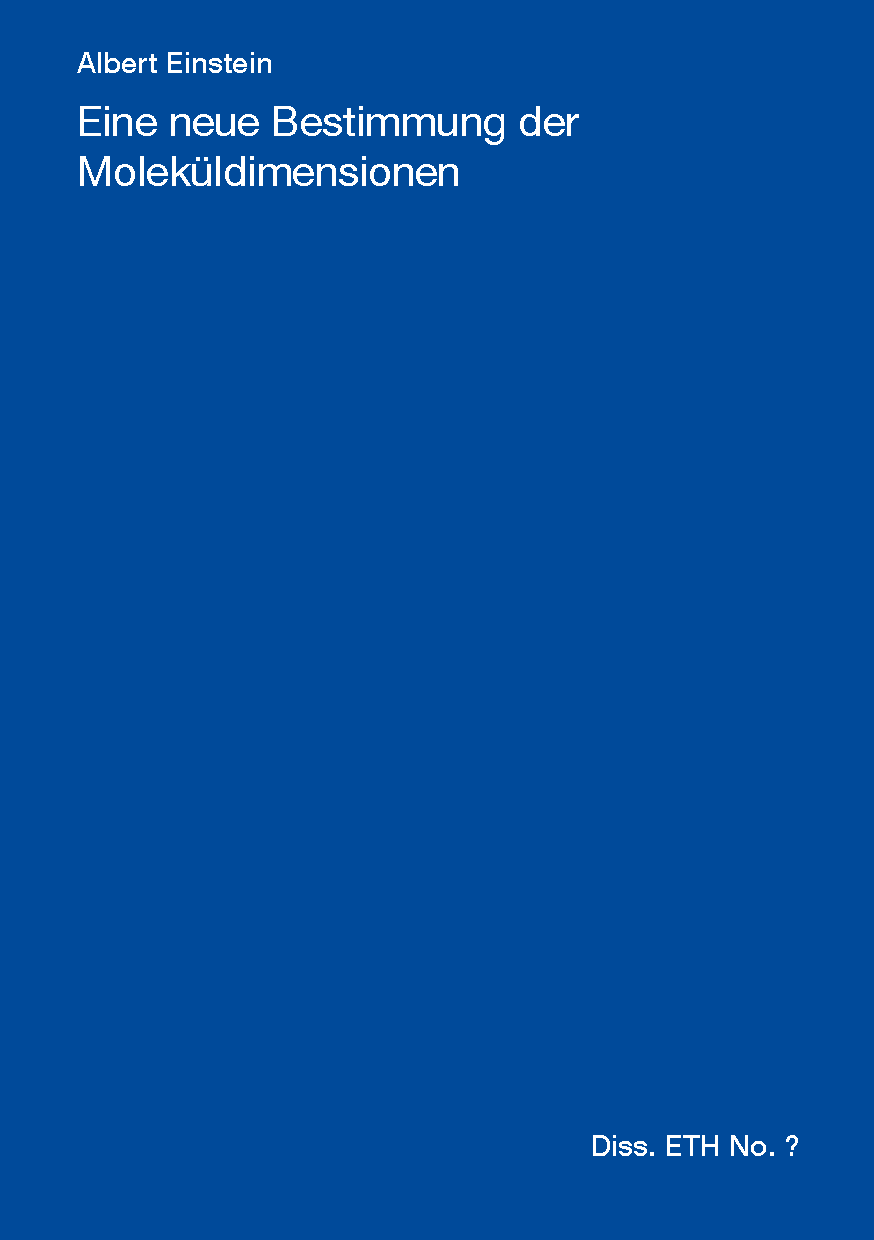
\includepdf[pages={1,{}}]{cover/crop/cover_front.pdf}
\cleardoublepage\setcounter{page}{1}

%********************************************************************
% Frontmatter
%*******************************************************
% \include{FrontBackmatter/DirtyTitlepage}
% \include{FrontBackmatter/Titlepage}
% \include{FrontBackmatter/Titleback}
% \cleardoublepage\include{FrontBackmatter/Dedication}
% %\cleardoublepage\include{FrontBackmatter/Foreword}
% \cleardoublepage\include{FrontBackmatter/Abstract}
% \cleardoublepage\include{FrontBackmatter/Publications}
% \cleardoublepage\include{FrontBackmatter/Acknowledgments}
% \cleardoublepage\include{FrontBackmatter/Contents}
%*******************************************************
% Little Dirty Titlepage
%*******************************************************
\thispagestyle{empty}
%*******************************************************
\begin{center}
    \spacedlowsmallcaps{\myName} \\ \medskip                        

    \begingroup
        \color{chapter-color}\spacedallcaps{\myTitle}
    \endgroup
\end{center}        

%*******************************************************
% Titlepage
%*******************************************************
\begin{titlepage}
	% if you want the titlepage to be centered, uncomment and fine-tune the line below (KOMA classes environment)
	%\begin{addmargin}[-1cm]{-3cm}
    \begin{center}
        \large
        \begingroup
            \spacedlowsmallcaps{Diss. ETH No. \myDissNumber}
        \endgroup

        \hfill

        \vfill

        \begingroup
            \spacedallcaps{\myTitle}
            %\spacedallcaps{\myTitleLineOne}\\
            %\spacedallcaps{\myTitleLineTwo}\\
            %\spacedallcaps{\myTitleLineThree}
        \endgroup

        \vfill

        \begingroup
            A dissertation submitted to attain the degree of\\
            \vspace{0.5em}
            \spacedlowsmallcaps{Doctor of Sciences}
            of
            \spacedlowsmallcaps{ETH Zurich} \\
            (Dr.\ sc.\ ETH Zurich)
        \endgroup

        \vfill

        \begingroup
            presented by\\
            \vspace{0.5em}
            \spacedlowsmallcaps{\myName}\\
            Dipl., Eidgenössisches Polytechnikum \\
            \vspace{0.5em}
            born on 14 March 1879\\
            citizen of Switzerland
        \endgroup

        \vfill

        \begingroup
            accepted on the recommendation of\\
            \vspace{0.5em}
            Prof.\ Dr.\ A. Kleiner, examiner\\
            Prof.\ Dr.\ H. Burkhardt, co-examiner
        \endgroup

        \vfill

        \myTime%

        \vfill
    \end{center}
  %\end{addmargin}
\end{titlepage}

\thispagestyle{empty}

\hfill

\vfill

\noindent\myName: \textit{\myTitle,} %\mySubtitle, %\myDegree, 
\textcopyright\ \myTime

\bigskip

\noindent\spacedlowsmallcaps{DOI}: \myDOI

%\bigskip
%
%\noindent\spacedlowsmallcaps{Supervisors}: \\
%\myProf \\
%\myOtherProf \\ 
%\mySupervisor
%
%\medskip
%
%\noindent\spacedlowsmallcaps{Location}: \\
%\myLocation
%
%\medskip
%
%\noindent\spacedlowsmallcaps{Time Frame}: \\
%\myTime

\cleardoublepage%*******************************************************
% Dedication
%*******************************************************
\thispagestyle{empty}
%\phantomsection
\refstepcounter{dummy}
%\pdfbookmark[1]{Dedication}{Dedication}

\vspace*{3cm}

\begin{center}
    To Mileva
\end{center}

\medskip

\cleardoublepage%*******************************************************
% Abstract
%*******************************************************
%\renewcommand{\abstractname}{Abstract}
\pdfbookmark[1]{Abstract}{Abstract}
\begingroup
\let\clearpage\relax
\let\cleardoublepage\relax
\let\cleardoublepage\relax

\chapter*{Abstract}

English abstract here.

\endgroup

\cleardoublepage%

\begingroup
\let\clearpage\relax
\let\cleardoublepage\relax
\let\cleardoublepage\relax

\begin{otherlanguage}{ngerman}
\pdfbookmark[1]{Zusammenfassung}{Zusammenfassung}
\chapter*{Zusammenfassung}

Deutsche Zusammenfassung hier.

\end{otherlanguage}

\endgroup

\vfill
\cleardoublepage%*******************************************************
% Acknowledgments
%*******************************************************
\pdfbookmark[1]{Acknowledgements}{acknowledgements}

\bigskip

\begingroup
\let\clearpage\relax
\let\cleardoublepage\relax
\let\cleardoublepage\relax
\chapter*{Acknowledgements}

\def\thanks#1{%
\begingroup
\leftskip1em
\noindent #1
\par
\endgroup
}

I would like to thank \dots

\endgroup

\pagestyle{scrheadings}
\cleardoublepage%*******************************************************
% Table of Contents
%*******************************************************
%\phantomsection
\refstepcounter{dummy}
\pdfbookmark[1]{\contentsname}{tableofcontents}
\setcounter{tocdepth}{2} % <-- 2 includes up to subsections in the ToC
\setcounter{secnumdepth}{3} % <-- 3 numbers up to subsubsections
\manualmark%
\markboth{\spacedlowsmallcaps{\contentsname}}{\spacedlowsmallcaps{\contentsname}}
\tableofcontents
\automark[section]{chapter}
\renewcommand{\chaptermark}[1]{\markboth{\spacedlowsmallcaps{#1}}{\spacedlowsmallcaps{#1}}}
\renewcommand{\sectionmark}[1]{\markright{\thesection\enspace\spacedlowsmallcaps{#1}}}
%*******************************************************
% List of Figures and of the Tables
%*******************************************************
\clearpage

\begingroup
    \let\clearpage\relax
    \let\cleardoublepage\relax
    \let\cleardoublepage\relax
    %*******************************************************
    % List of Figures
    %*******************************************************
    %\phantomsection
    % \refstepcounter{dummy}
    %\addcontentsline{toc}{chapter}{\listfigurename}
    % \pdfbookmark[1]{\listfigurename}{lof}
    % \listoffigures

    % \vspace{8ex}

    %*******************************************************
    % List of Tables
    %*******************************************************
    %\phantomsection
    % \refstepcounter{dummy}
    %\addcontentsline{toc}{chapter}{\listtablename}
    % \pdfbookmark[1]{\listtablename}{lot}
    % \listoftables

    % \vspace{8ex}
    % \newpage

    %*******************************************************
    % List of Listings
    %*******************************************************
      %\phantomsection
    %\refstepcounter{dummy}
    %\addcontentsline{toc}{chapter}{\lstlistlistingname}
    %\pdfbookmark[1]{\lstlistlistingname}{lol}
    %\lstlistoflistings%

    %\vspace{8ex}

    % Notation
    \refstepcounter{dummy}
    \pdfbookmark[1]{Notation}{notation}
    \markboth{\spacedlowsmallcaps{Notation}}{\spacedlowsmallcaps{Notation}}
    \chapter*{Notation}

    \section*{Frequently used symbols}%
    \vskip -2em
    \begin{tabularx}{\textwidth}{lX}
      %\toprule%
      %\tableheadline{Symbol} & \tableheadline{Meaning} \\
      %\midrule%
      $E$ & energy \\
      $m$ & rest mass \\
      $p$ & impulse \\
      %\bottomrule
    \end{tabularx}

    \section*{Physical constants}
    \sisetup{separate-uncertainty=false}
    \vskip -2em
    \begin{tabularx}{\textwidth}{lX}
$c$ & speed of light in vacuum, $c=\u{299792458}{\metre\per\second}$ \\
    \end{tabularx}
    \begin{flushright}
    (CODATA 2014~\cite{codata})
    \end{flushright}
    \sisetup{separate-uncertainty=true}
\endgroup


%********************************************************************
% Mainmatter
%*******************************************************
\cleardoublepage
\pagestyle{scrheadings}
\pagenumbering{arabic}
%\setcounter{page}{90}
% use \cleardoublepage here to avoid problems with pdfbookmark
\cleardoublepage
\chapter{Introduction}
\label{ch:introduction}

\dictum[Immanuel Kant]{%
  Sapere aude! Habe Mut, dich deines eigenen Verstandes zu bedienen! }%
\vskip 1em

\begin{otherlanguage}{ngerman}
Die ältesten Bestimmungen der wahren Grösse der Moleküle hat die kinetische
Theorie der Gase ermöglicht, während die an Flüssigkeiten beobachteten
physikalischen Phänomene bis jetzt zur Bestimmung der Molekülgrössen nicht
gedient haben. \dots
\end{otherlanguage}


% \part{Some Kind of Manual}\label{pt:manual}
% \include{Chapters/Chapter01}
% \cleardoublepage
% \ctparttext{You can put some informational part preamble text here.
% Illo principalmente su nos. Non message \emph{occidental} angloromanic
% da. Debitas effortio simplificate sia se, auxiliar summarios da que,
% se avantiate publicationes via. Pan in terra summarios, capital
% interlingua se que. Al via multo esser specimen, campo responder que
% da. Le usate medical addresses pro, europa origine sanctificate nos se.}
% \part{The Showcase}\label{pt:showcase}
% \include{Chapters/Chapter02}
% %\addtocontents{toc}{\protect\clearpage} % <--- just debug stuff, ignore
% \include{Chapters/Chapter03}
% %\include{multiToC} % <--- just debug stuff, ignore for your documents
% ********************************************************************
% Backmatter
%*******************************************************
\appendix
%\renewcommand{\thechapter}{\alph{chapter}}
\cleardoublepage
\part{Appendix}
\include{Chapters/Chapter0A}
%********************************************************************
% Other Stuff in the Back
%*******************************************************
\pdfbookmark[-1]{Back Matter}{back} % Dummy part bookmark for back matter
\cleardoublepage\include{FrontBackmatter/Bibliography}
\cleardoublepage\include{FrontBackmatter/Declaration}
\cleardoublepage\include{FrontBackmatter/Colophon}
% ********************************************************************
% Game Over: Restore, Restart, or Quit?
%*******************************************************
\end{document}
% ********************************************************************